\chapter{Arhitektura i dizajn sustava}

Arhitektura sustava može se podijeliti na tri ključna podsustava:

\begin{packed_enum}
	\item Web poslužitelj:
	\begin{packed_enum}
		\item Ključan dio web aplikacije.
		\item Odgovoran za interakciju između klijenta i aplikacije.
		\item Koristi HTTP/HTTPS protokol za prijenos informacija na webu.
		\item Inicira pokretanje web aplikacije i proslijeđuje zahtjeve.
	\end{packed_enum}
	\item Web aplikacija:
	\begin{packed_enum}
		\item Procesira korisničke zahtjeve i obrađuje ih.
		\item Pristupa bazi podataka prema potrebi.
		\item Generira odgovore u obliku HTML dokumenata za prikaz u web pregledniku.
	\end{packed_enum}			
	\item Baza podataka:	
	\begin{packed_enum}
		\item Sprema podatke koji se koriste ili modificiraju unutar web aplikacije.
	\end{packed_enum}
\end{packed_enum}

Korisnik, putem web preglednika, šalje zahtjeve web poslužitelju. 
Web poslužitelj zatim inicira rad web aplikacije, koja procesira zahtjeve, pristupa bazi podataka po potrebi i vraća odgovore u obliku HTML dokumenata. 
Ova interakcija omogućuje korisnicima pregled i manipulaciju sadržajem putem web sučelja.

\begin{figure}[H]
	\includegraphics[scale=0.5]{slike/arhitektura.png}
	\centering
	\caption{Arhitektura sustava}
	\label{fig:arhitektura}
\end{figure}

Za izradu ovog projekta koristili smo se Spring Boot frameworkom u Javi kroz
razvojno okruženje IntelliJ Community Edition, Javascriptom uz React u Visual
Studio Code-u te drugim programima za dizajn slika i grafova ( AstahUML itd.).


 Spring Boot podržava koncept MVC, odnosno Model-Pogled-Nadglednik
(engl. \textit{Model View Controller}), arhitekture, tj. stilističke varijacije arhitekture zasnovane 
na događajima. Takve arhitekture odlikuje to što se komponente međusobno ne pozivaju
eksplicitno, već neke od njih generiraju signale (događaje) ne znajući koja druga
"osluškuje" tj. očekuje takav signal i na njega reagira. To se postiže kroz Spring Web MVC modul. 
\begin{packed_item}
	\item Model: Spring Boot omogućava korištenje Java objekata kao modela. Ovi objekti predstavljaju podatke koji se koriste u aplikaciji.
	Spring Data može se integrirati za jednostavno upravljanje podacima i komunikaciju s bazom podataka.
	\item View: Spring Boot pruža fleksibilnost u odabiru tehnologije za prikazivanje korisničkog sučelja. Prikazi se često implementiraju kroz HTML datoteke, a moguće je koristiti različite template engines (Thymeleaf, FreeMarker, JSP).
	Pomoću konfiguracija view resolvera jednostavno se integriraju odabrane tehnologije za prikazivanje podataka korisnicima.
	\item Controller: Anotacije poput @Controller i @RestController omogućuju jednostavno označavanje klasa koje djeluju kao kontroleri.
	@RequestMapping i slične anotacije omogućuju mapiranje HTTP zahtjeva na određene metode kontrolera.
	Spring Boot automatski prepoznaje i konfigurira komponente kontrolera.		
\end{packed_item}

Kod MVC-a pogodno je što smanjuje međuovisnost korisničkog sučelja i ostatka sustava, a omogućuje i nezavisan razvoj, nadogradnje i dodavanje različitih dijelova aplikacije. Sadrži različite
gotove predloške za klase koji nam olakšavaju proces izrade.
				
		\section{Baza podataka}
			    


		Baze podataka neizostavan su dio razvoja programske potpore jer danas gotova svaka domena primjene 
		obiluje mnoštvom podataka koje treba pohraniti na organiziran način kako bi se efikasno dohvaćali,
		 mijenjali i nadopunjavali. Za upravljanje bazom podataka mogu se koristiti različiti sustavi koji 
		 obavljaju optimiranje upita i omogućuju rukovanje podatcima. Mi smo odlučili koristiti PostgreSQL 
		 koji nam je bio preporučen na kolegiju Baze podataka. \newline Relacijski nam model baze podataka 
		 omogućuje vjeran prikaz stvarnosti pomoću relacija u koje pohranjujemo vrijednosti odabranih 
		 atributa vezanih uz entitete bitne za domenu primjene. Atributi su imenovani stupci te tablice. ER (Entity-Relationship) model podataka zadržava dobra svojstva relacijskog modela, a uz to omogućuje eksplicitni prikaz semantičkih informacija vezanih uz veze (odnose) između entiteta. Kako bismo prikazali kako su eniteti našeg sustava povezani koristit ćemo ER model baze podataka.
za podataka ove aplikacije sastoji se od sljedećih entiteta:
		\begin{packed_item}
			\item Korisnik
			\item Pozicija tragača
			\item Uloga
			\item Zadatak 
			\item Pripada postaji
			\item Osposobljen za
			\item Akcija
			\item Postaja
			\item Prijevozno sredstvo
			\item Komentar korisnika 
			\item Životinja
			\item Pozicija životinje
		\end{packed_item}

		\eject
			\subsection{Opis tablica}
			
					\textbf {Zadatak} Ovaj entitet sadrži sve važne informacije o zadatcima koje obavljaju tragači tijekom akcije, a stvaraju istraživači. Sadrži
				atribute: šifra zadatka, korisničko ime, tekst, završen, šifra akcije, šifra životinje i šifra vozila. 
				Ova tablica je u vezi s tablicom Prijevozno sredstvo preko tablice Osposobljen za te izravno preko 
				dentifikatora vozila(šifra vozila), s tablicom Akcija izravno preko identifikatora akcije (šifra akcije), 
				s tablicom Životinja izravno preko identifikatora životinje (šifra životinje).
				
				\begin{longtblr}[
					label=none,
					entry=none
					]{
						width = \textwidth,
						colspec={|X[6,l]|X[6, l]|X[20, l]|}, 
						rowhead = 1,
					} %definicija širine tablice, širine stupaca, poravnanje i broja redaka naslova tablice
					\hline \SetCell[c=3]{c}{\textbf{Zadatak}}	 \\ \hline[3pt]
					\SetCell{LightGreen} Šifra Zadatka & INT	&  	Jedinstveni brojčani identifikator zadatka  	\\ \hline
					\SetCell{LightGreen} Korisničko ime & VARCHAR	& 	Korisničko ime korisnika\\ \hline
					Tekst	& VARCHAR & Opis zadatka  	\\ \hline 
					Završen & BOOLEAN & Status je li zadatak završen  \\ \hline 
          \SetCell{LightBlue} Šifra akcije 	& INT & Jedinstveni brojčani identifikator akcije   	\\ \hline 
          \SetCell{LightBlue} Šifra životinje 	& INT &   Jedinstveni brojčani identifikator životinje  	\\ \hline 
          \SetCell{LightBlue} Šifra vozila 	& INT &  Jedinstveni brojčani identifikator vozila 	\\ \hline 
				\end{longtblr}

				\textbf {Akcija} Ovaj entitet sadrži sve važne informacije o akcijama pretraživanja i praćenja. Sadrži
			atribute: šifra akcije, naziv akcije, aktivna i korisničko ime. 
			Ova tablica je u vezi s tablicom Korisnik preko identifikatora korisnika(korisničko ime),
			 s tablicom Životinja preko tablice Komentar korisnika, s tablicom Zadatak i tablicom Pozicija tragača.
				
				\begin{longtblr}[
					label=none,
					entry=none
					]{
						width = \textwidth,
						colspec={|X[6,l]|X[6, l]|X[20, l]|}, 
						rowhead = 1,
					} %definicija širine tablice, širine stupaca, poravnanje i broja redaka naslova tablice
          \hline \SetCell[c=3]{c}{\textbf{Akcija}}	 \\ \hline[3pt]
					\SetCell{LightGreen} Šifra akcije & INT	&  	Jedinstveni ključ za identifikaciju zadatka  	\\ \hline
					Naziv akcije	& VARCHAR &  Puni naziv akcije  	\\ \hline 
					Aktivna & BOOLEAN & Status je li akcija aktvna  \\ \hline 
          \SetCell{LightBlue} Korisničko ime 	& VARCHAR &  Korisničko ime korisnika 	\\ \hline 
				\end{longtblr}
			
				\textbf {Komentar korisnika} Ovaj entitet sadrži informacije o komentarima korisnika o praćenoj životinji 
				koje mogu ostaviti tijekom akcije. Sadrži atribute: šifra životinje, korisničko ime, šifra akcije i komentar. 
		

				\begin{longtblr}[
					label=none,
					entry=none
					]{
						width = \textwidth,
						colspec={|X[6,l]|X[6, l]|X[20, l]|}, 
						rowhead = 1,
					} %definicija širine tablice, širine stupaca, poravnanje i broja redaka naslova tablice
          \hline \SetCell[c=3]{c}{\textbf{Komentar korisnika}}	 \\ \hline[3pt]
					\SetCell{LightGreen} Šifra životinje & INT	&  	Jedinstveni brojčani identifikator zadatka  	\\ \hline
					\SetCell{LightGreen} Korisničko ime & VARCHAR	&  	Korisničko ime korisnika 	\\ \hline
					\SetCell{LightGreen} Šifra akcije & INT	&  	Jedinstveni brojčani identifikator akcije  	\\ \hline
					Komentar	& VARCHAR & Sadržaj komentara  	\\ \hline 
				\end{longtblr}
				
				\textbf {Životinja} Ovaj entitet sadrži sve važne informacije o životinjama. Sadrži
			atribute: šifra životinje, naziv , latinski naziv i opis. 
			Ova tablica povezana je s tablicom Pozicija životinje s tablicom Zadatak preko identifikatora životinje(šifra životinje) te s tablicom Akcija

				\begin{longtblr}[
					label=none,
					entry=none
					]{
						width = \textwidth,
						colspec={|X[6,l]|X[6, l]|X[20, l]|}, 
						rowhead = 1,
					} %definicija širine tablice, širine stupaca, poravnanje i broja redaka naslova tablice
          \hline \SetCell[c=3]{c}{\textbf{Životinja}}	 \\ \hline[3pt]
					\SetCell{LightGreen} Šifra životinje & INT	&  	Jedinstveni brojčani identifikator životinje  	\\ \hline
					Naziv	& VARCHAR & Puni naziv životinje  	\\ \hline 
					Latinski naziv	& VARCHAR & Latinski naziv životinje  	\\ \hline 
					Opis	& VARCHAR & Sadržaj komentara  	\\ \hline 
				\end{longtblr}

				\textbf {Pozicija životinje} Ovaj entitet sadrži informacije o poziciji životinje. 
				Pomoću njega bilježimo gibanje životinje na kartama. Sadrži
			atribute: šifra životinje, vremenska oznaka, geografska širina i geografska dužina.


				\begin{longtblr}[
					label=none,
					entry=none
					]{
						width = \textwidth,
						colspec={|X[6,l]|X[6, l]|X[20, l]|}, 
						rowhead = 1,
					} %definicija širine tablice, širine stupaca, poravnanje i broja redaka naslova tablice
          \hline \SetCell[c=3]{c}{\textbf{Pozicija životinje}}	 \\ \hline[3pt]
					\SetCell{LightGreen} Šifra životinje & INT	&  	Jedinstveni brojčani identifikator životinje \\ \hline
					\SetCell{LightGreen} Vremenska oznaka & TIMESTAMP	&  	Zadnje vrijeme u kojem je viđena životinja  	\\ \hline
          Geografska širina	& DOUBLE & Iznos geografske širine  	\\ \hline 
          Geografska dužina	& DOUBLE & Iznos geografske dužine  	\\ \hline 
				\end{longtblr}

				\textbf {Pozicija tragača} Ovaj entitet sadrži informacije o poziciji tragača. 
				Pomoću njega bilježimo kretanje tragača na kartama. Sadrži
			atribute: korisničko ime, vremenska oznaka, šifra akcije, geografska širina i geografska dužina.

				\begin{longtblr}[
					label=none,
					entry=none
					]{
						width = \textwidth,
						colspec={|X[6,l]|X[6, l]|X[20, l]|}, 
						rowhead = 1,
					} %definicija širine tablice, širine stupaca, poravnanje i broja redaka naslova tablice
          \hline \SetCell[c=3]{c}{\textbf{Pozicija tragača}}	 \\ \hline[3pt]
					\SetCell{LightGreen} Korisničko ime & VARCHAR	&  	Korisničko ime korisnika  	\\ \hline
					\SetCell{LightGreen} Vremenska oznaka & TIMESTAMP	&  	Zadnje vrijeme kada je tragač zabilježio svoju poziciju  	\\ \hline
					\SetCell{LightGreen} Šifra akcije & INT	&  	Jedinstveni brojčani identifikator akcije  	\\ \hline
          Geografska širina	& DOUBLE & Iznos geografske širine  	\\ \hline 
          Geografska dužina	& DOUBLE & Iznos geografske dužine  	\\ \hline 
				\end{longtblr}

				\textbf {Korisnik} Ovaj entitet sadrži sve važne informacije o korisnicima. Sadrži
			atribute: korisničko ime, email, lozinka, ime, prezime, fotografija i šifra uloge.
			Ova tablica je u vezi s tablicama Akcija, Pozicija tragača, Uloga i Komentar korisnika.

				\begin{longtblr}[
					label=none,
					entry=none
					]{
						width = \textwidth,
						colspec={|X[6,l]|X[6, l]|X[20, l]|}, 
						rowhead = 1,
					} %definicija širine tablice, širine stupaca, poravnanje i broja redaka naslova tablice
          \hline \SetCell[c=3]{c}{\textbf{Korisnik}}	 \\ \hline[3pt]
					\SetCell{LightGreen} Korisničko ime & VARCHAR	&  	Ime korisnika  	\\ \hline
          Email	& VARCHAR & Sadržaj komentara  	\\ \hline 
          Lozinka & VARCHAR & Lozinka korisnika \\ \hline
          Ime & VARCHAR & Ime korisnika \\ \hline
          Prezime & VARCHAR & Prezime korisnika \\ \hline
          Fotografija & VARCHAR & Fotografija korisnika \\ \hline
          \SetCell{LightBlue} Šifra uloge 	& INT &   Jedinstveni brojčani identifikator uloge	\\ \hline 

				\end{longtblr}

				\textbf {Pripada postaji} Ova veza sadrži informacije po kojima saznajemo koji korisnik pripada kojoj postaji.
				Povezuje entitete Korisnik i Postaja te sadrži njihove ključne atribute: korisničko ime i šifra postaje.

				\begin{longtblr}[
					label=none,
					entry=none
					]{
						width = \textwidth,
						colspec={|X[6,l]|X[6, l]|X[20, l]|}, 
						rowhead = 1,
					} %definicija širine tablice, širine stupaca, poravnanje i broja redaka naslova tablice
          \hline \SetCell[c=3]{c}{\textbf{Pripada postaji}}	 \\ \hline[3pt]
					\SetCell{LightGreen} Korisničko ime & VARCHAR	&  	Korisničko ime korisnika  	\\ \hline
					\SetCell{LightGreen} Šifra postaje & VARCHAR	&  	Jedinstveni brojčani identifikator postaje\\ \hline

				\end{longtblr}

				\textbf {Postaja} Ovaj entitet sadrži informacije o postajama. Sastoji se od
			atributa: šifra postaje i naziv postaje.

				\begin{longtblr}[
					label=none,
					entry=none
					]{
						width = \textwidth,
						colspec={|X[6,l]|X[6, l]|X[20, l]|}, 
						rowhead = 1,
					} %definicija širine tablice, širine stupaca, poravnanje i broja redaka naslova tablice
          \hline \SetCell[c=3]{c}{\textbf{Postaja}}	 \\ \hline[3pt]
					\SetCell{LightGreen} Šifra postaje & VARCHAR	&  	Jedinstveni brojčani identifikator korisnika \\ \hline
					Naziv postaje & VARCHAR	&  	Pun naziv postaje  	\\ \hline

				\end{longtblr}

				\textbf {Osposobljen za} Ova veza sadrži informacije po kojima saznajemo koji korisnik ima sposobnosti za voziti koje prijevozno sredstvo.
				Povezuje entitete Korisnik i Prijevozno sredstvo te sadrži njihove ključne atribute: korisničko ime i šifra vozila.

				\begin{longtblr}[
					label=none,
					entry=none
					]{
						width = \textwidth,
						colspec={|X[6,l]|X[6, l]|X[20, l]|}, 
						rowhead = 1,
					} %definicija širine tablice, širine stupaca, poravnanje i broja redaka naslova tablice
          \hline \SetCell[c=3]{c}{\textbf{Osposobljen za}}	 \\ \hline[3pt]
					\SetCell{LightGreen} Korisničko ime & VARCHAR	&  	Ime korisnika  	\\ \hline
					\SetCell{LightGreen} Šifra vozila & INT	&   Jedinstveni brojčani identifikator vozila  	\\ \hline

				\end{longtblr}

				\textbf {Prijevozno sredstvo} Ovaj entitet sadrži informacije o vozilima za koje tragači mogu biti osposobljeni.
				 Sastoji se od atributa: šifra vozila i naziv vozila.


				\begin{longtblr}[
					label=none,
					entry=none
					]{
						width = \textwidth,
						colspec={|X[6,l]|X[6, l]|X[20, l]|}, 
						rowhead = 1,
					} %definicija širine tablice, širine stupaca, poravnanje i broja redaka naslova tablice
          \hline \SetCell[c=3]{c}{\textbf{Prijevozno sredstvo}}	 \\ \hline[3pt]
					\SetCell{LightGreen} Šifra vozila & INT	&   Jedinstveni brojčani identifikator vozila  	\\ \hline
          Naziv vozila & VARCHAR & Puni naziv vozila \\ \hline

				\end{longtblr}

				\textbf {Uloga} Ovaj entitet sadrži informacije o ulogama korisnika. Sastoji se od
			atributa: šifra uloge i naziv uloge.


				\begin{longtblr}[
					label=none,
					entry=none
					]{
						width = \textwidth,
						colspec={|X[6,l]|X[6, l]|X[20, l]|}, 
						rowhead = 1,
					} %definicija širine tablice, širine stupaca, poravnanje i broja redaka naslova tablice
          \hline \SetCell[c=3]{c}{\textbf{Uloga}}	 \\ \hline[3pt]
          \SetCell{LightGreen} Šifra Uloge & INT	&  Jedinstveni brojčani identifikator uloge	\\ \hline
          Naziv uloge	& VARCHAR & Puni naziv uloge  	\\ \hline 

				\end{longtblr}

			\eject

			\subsection{Dijagram baze podataka}

			\begin{figure}[H]
				\includegraphics[scale=0.9]{slike/dijagram baze podataka.png} 
				\centering
				\caption{Dijagram baze podataka}
				\label{fig:dijagram_baze_podataka}
			\end{figure}
			
			\eject
			
			
		\section{Dijagram razreda}

		Na slikama \ref{fig:controllers}, \ref{fig:data_transfer_objects} i \ref{fig:models} su prikazani klasni dijagrami koji pripadaju backend dijelu MVC
		arhitekture. Razredi prikazani na slici \ref{fig:controllers} nasljeđuju Controller razred. 
		Metode implementirane u tim razredima manipuliraju s Data transfer object, a oni
		su dohvaćeni s pomoću metoda u Model razredima. 

		Metode unutar Controller razreda vraćaju JSON datoteke.
		Razredi su logički podijeljeni prema pravu pristupa metodama specifičnih aktora kako bi se smanjila prenapučenost unutar dijagrama.
		Pri prikazu su naglašene samo ovisnosti između razreda koji pripadaju istom dijelu dijagrama radi jednostavnije organizacije.
		Vrsta ovisnosti između različitim razredima može se zaključiti iz naziva i tipova atributa unutar tih razreda.
		Controller razredi sadrži privatne varijable koje mu omogućuju komunikaciju sa Service razredima.
		
		\eject

			\begin{figure}[H]
				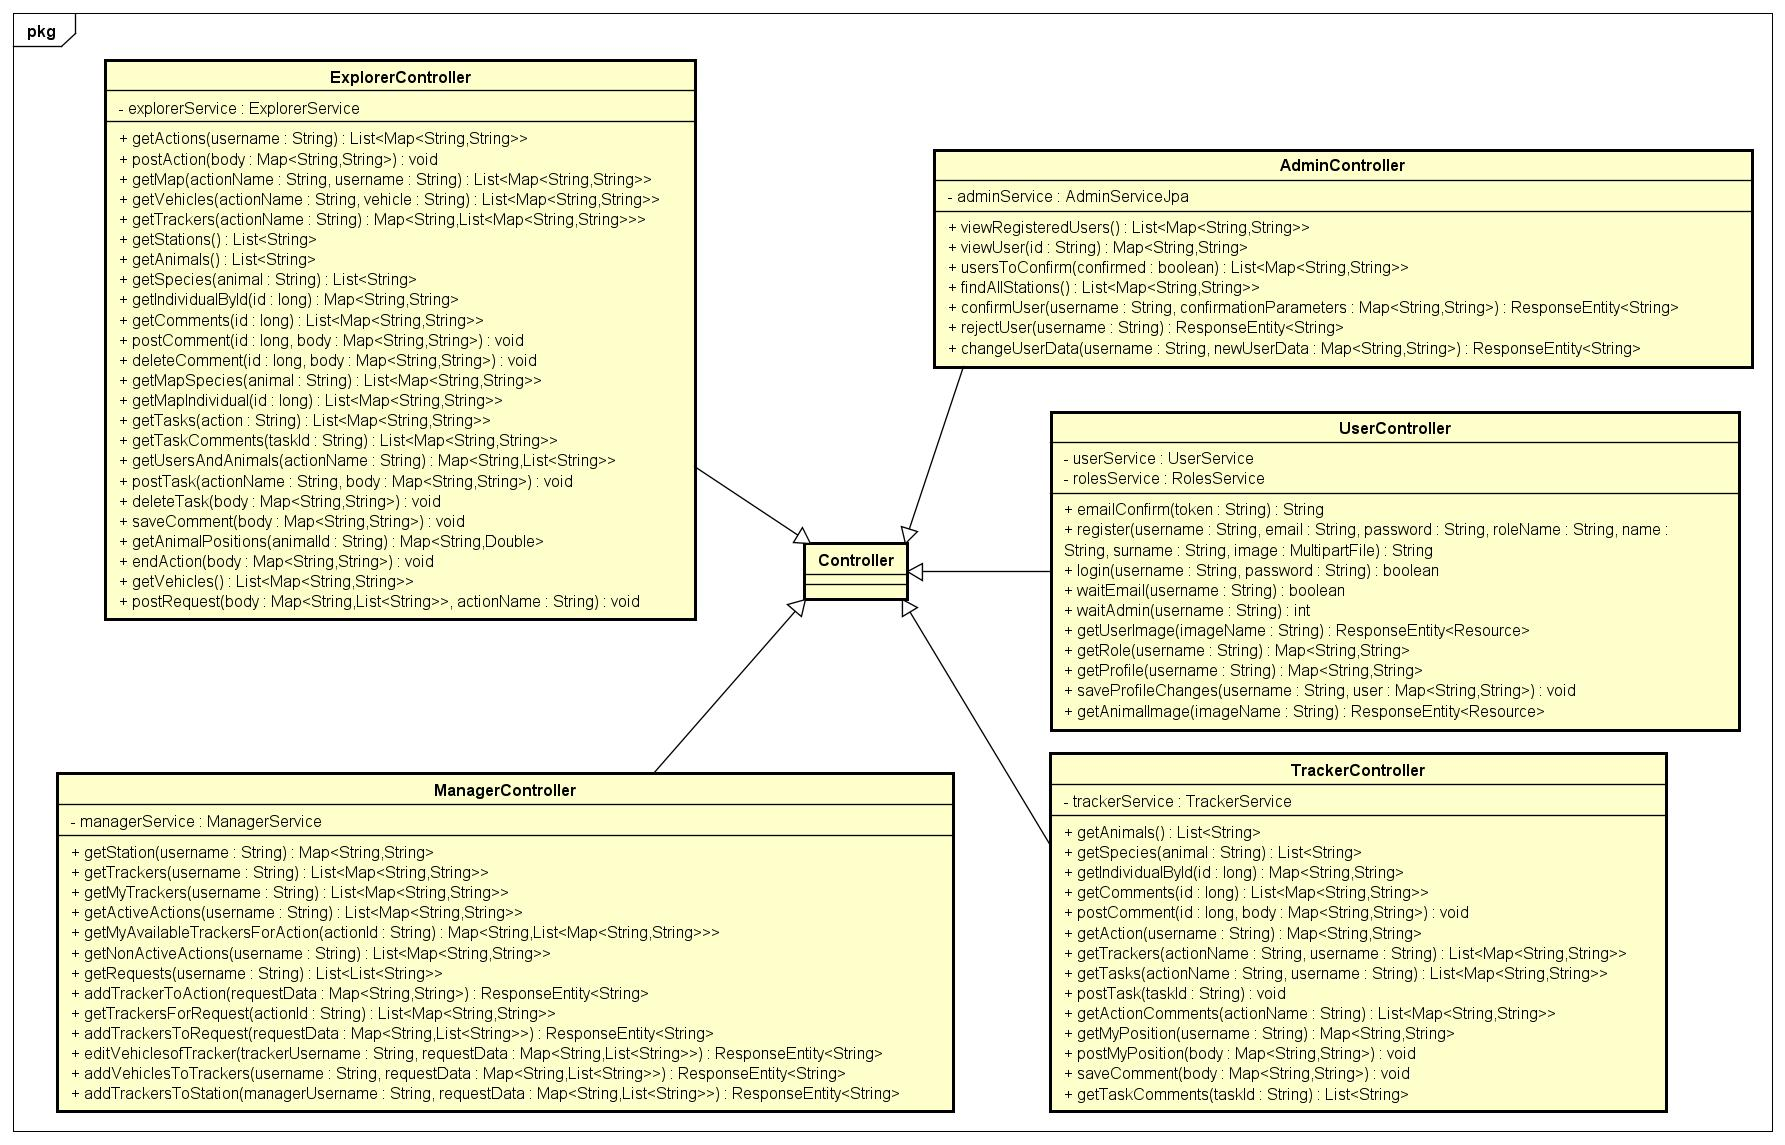
\includegraphics[scale=0.23]{slike/klasni_dijagram_controllers.jpg}
				\centering
				\caption{Dijagram razreda - dio Controllers}
				\label{fig:controllers}
			\end{figure}
			
			\eject

			\begin{figure}[H]
				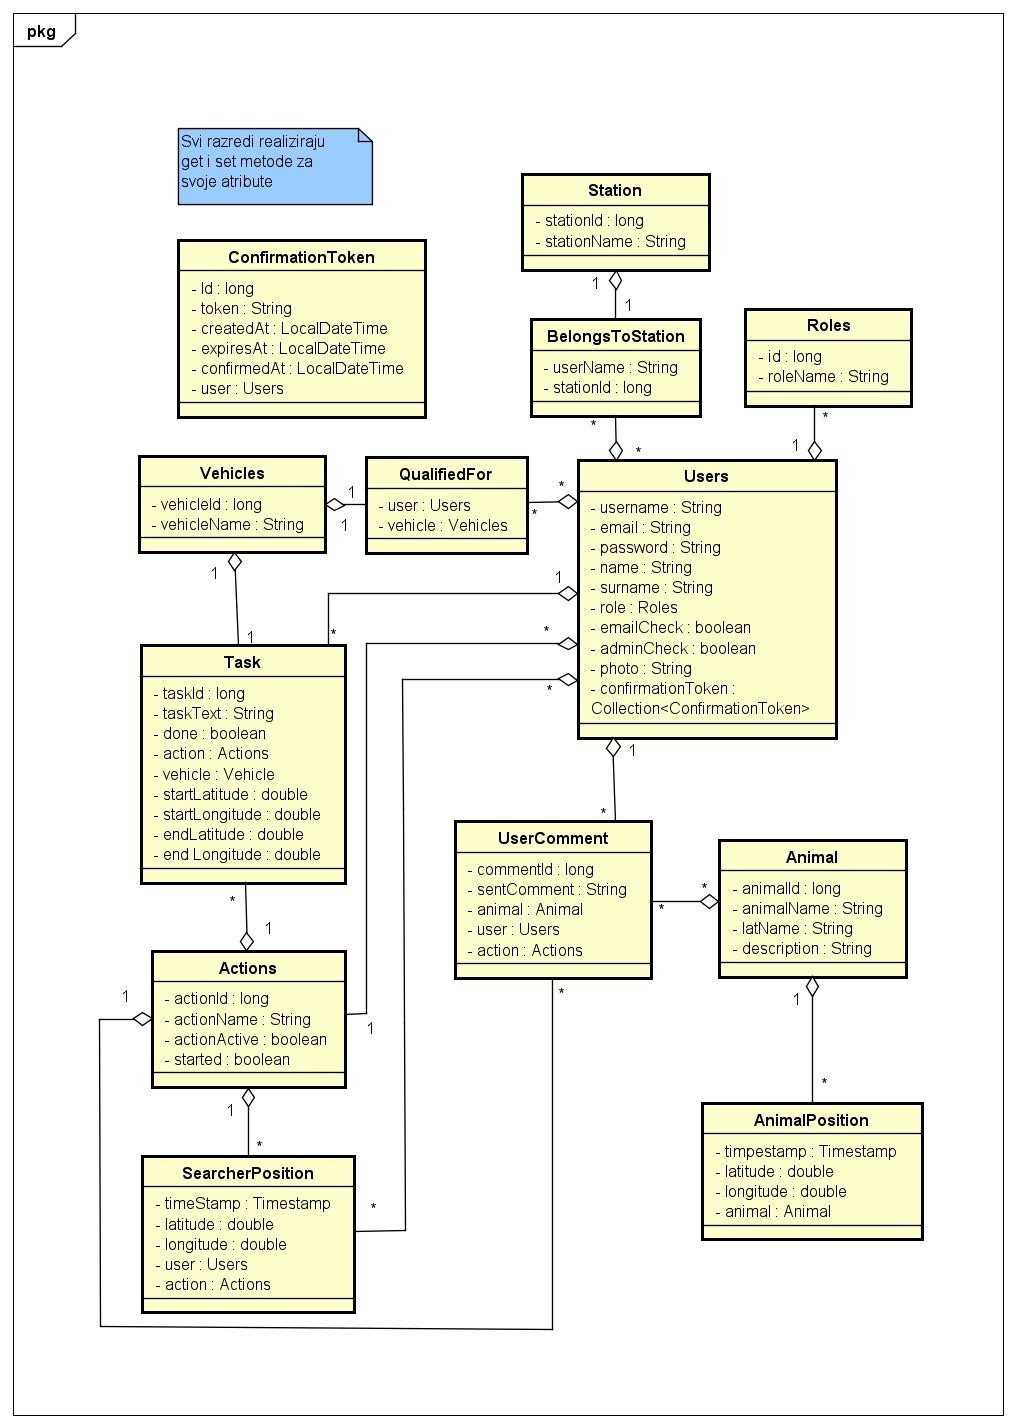
\includegraphics[scale=0.35]{slike/klasni_dijagram_DTO.jpg}
				\centering
				\caption{Dijagram razreda - dio Data transfer objects}
				\label{fig:data_transfer_objects}
			\end{figure}

			Model razredi prikazuju strukturu baze podataka u aplikaciji. 
			Implementirane metode komuniciraju s bazom podataka te vraćaju tražene podatke. 
			Razred Users predstavlja neregistriranog korisnika koji se može registrirati u 
			sustav unošenjem informacija.


			\eject

			\begin{figure}[H]
				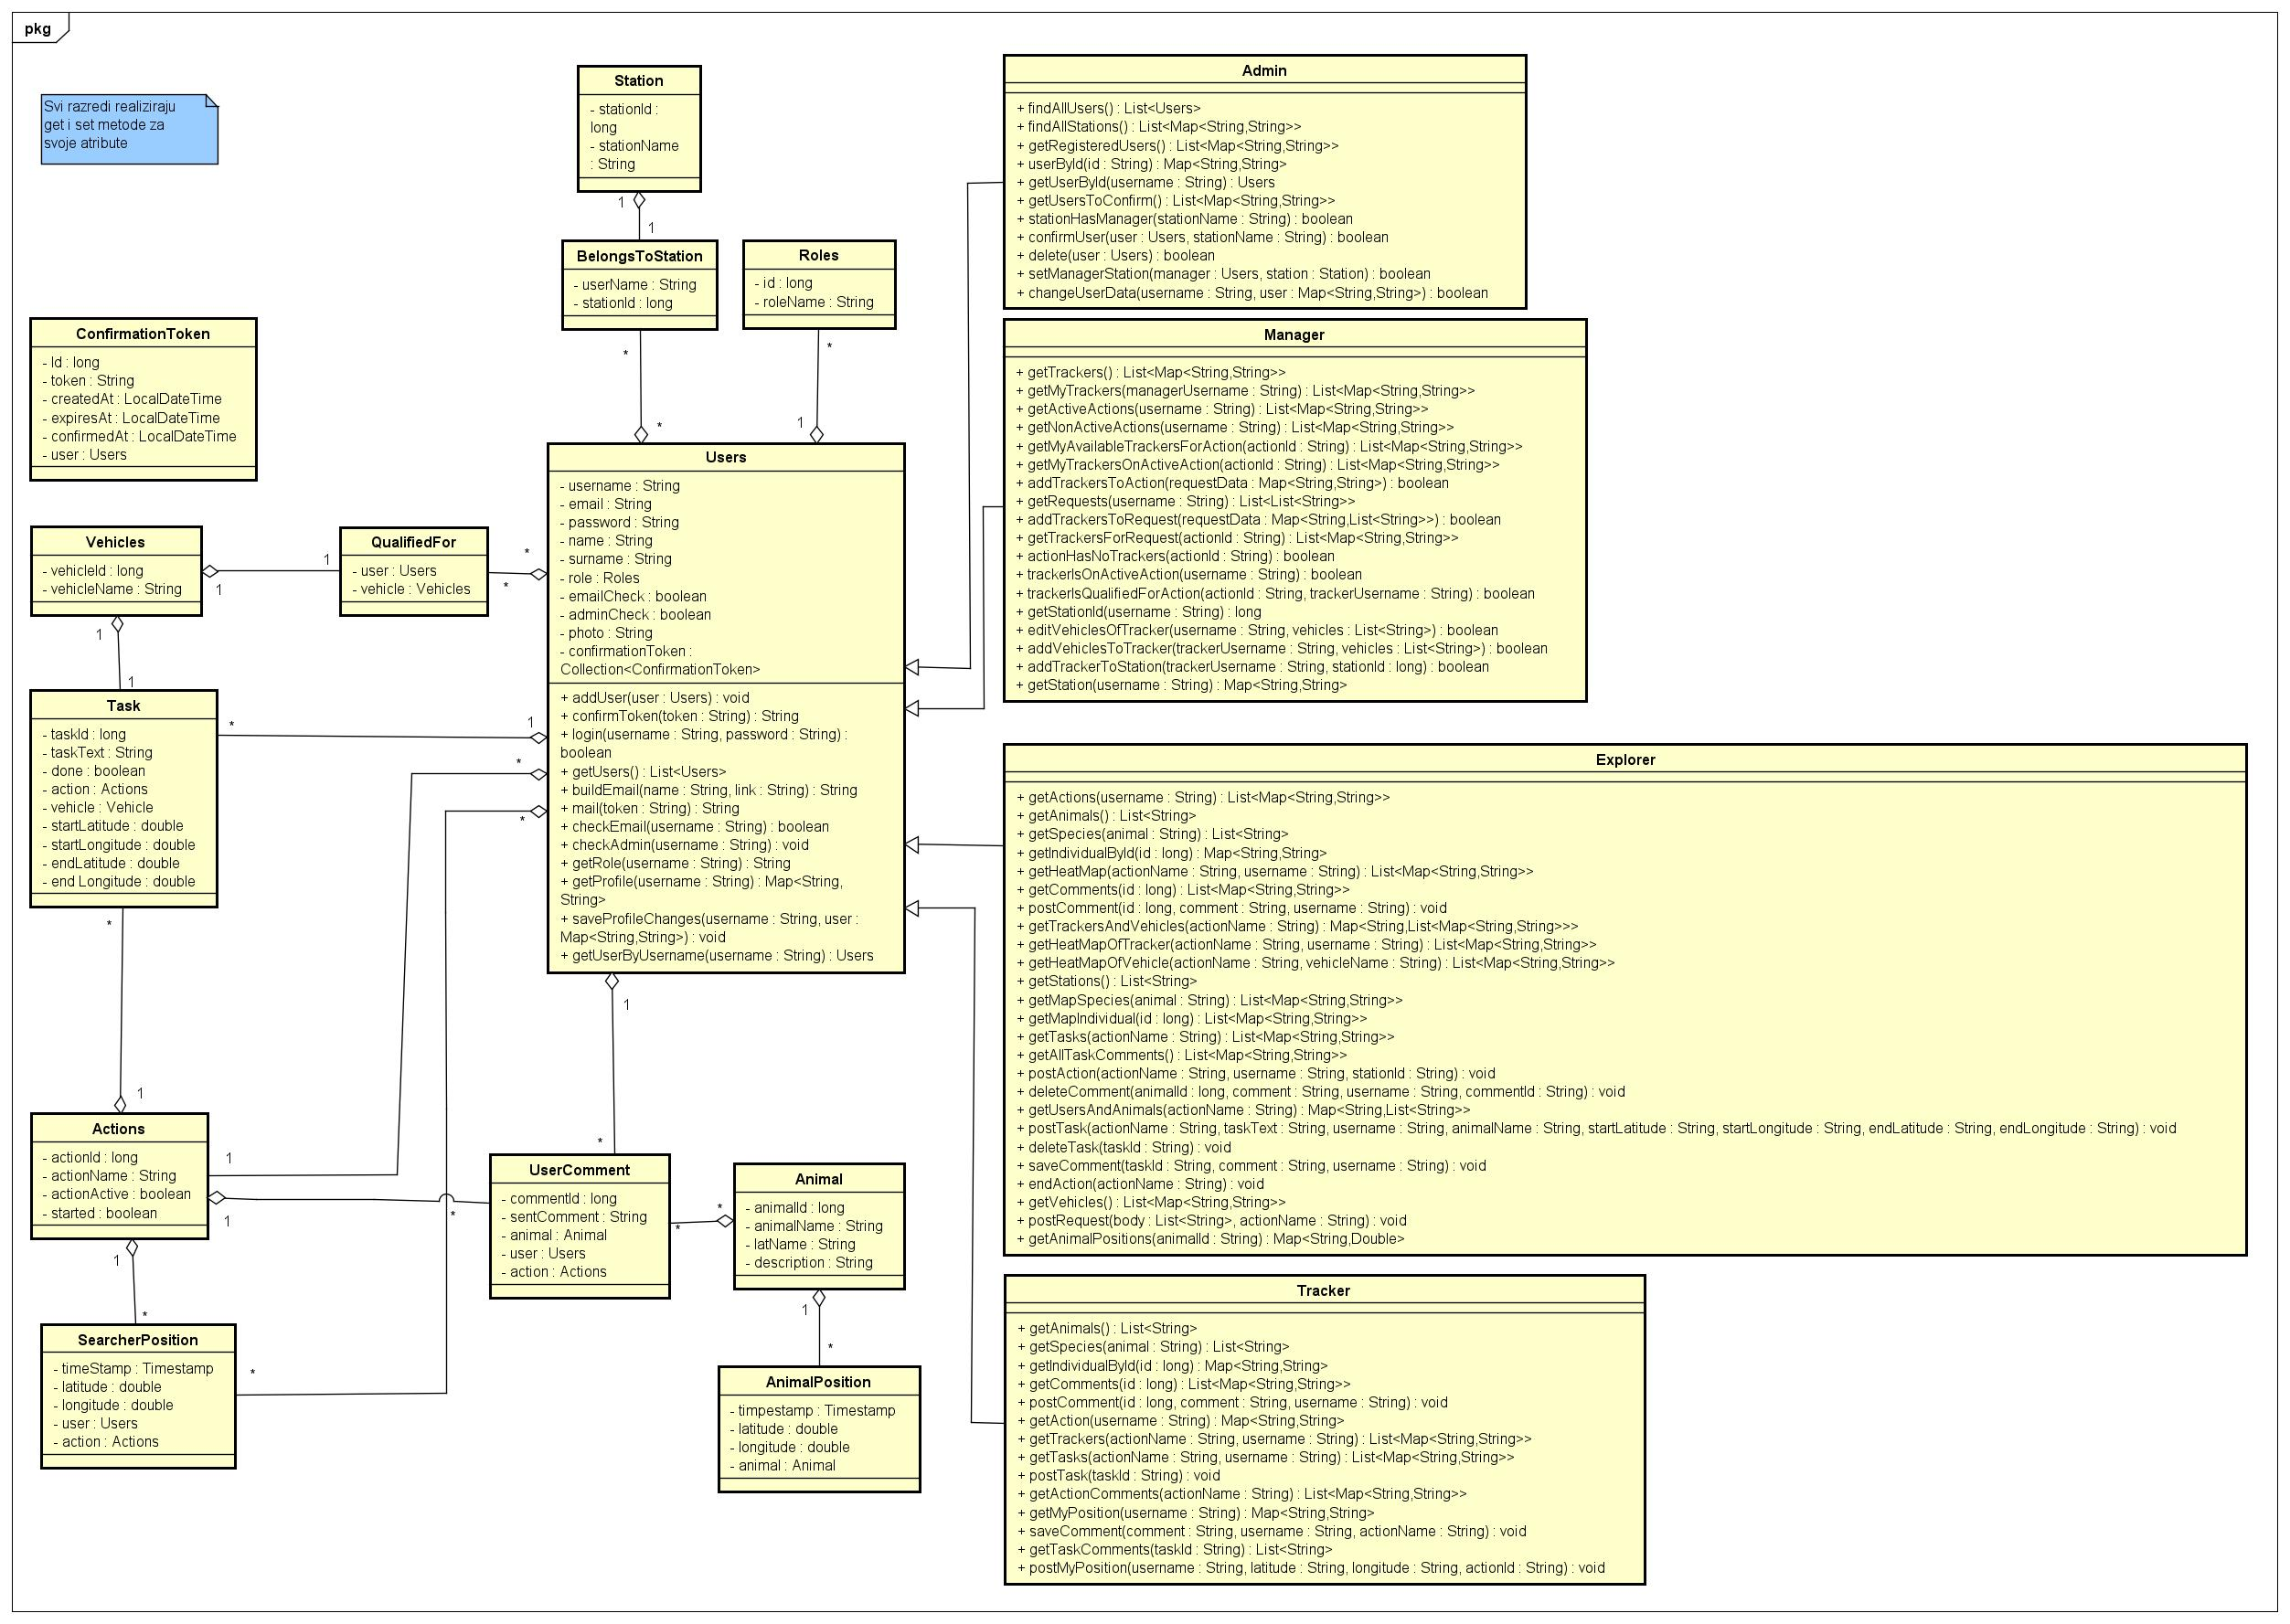
\includegraphics[scale=0.15]{slike/klasni_dijagram_models.jpg}
				\centering
				\caption{Dijagram razreda - dio Models}
				\label{fig:models}
			\end{figure}
			
			
			
			\eject
		
		\section{Dijagram stanja}
			
			Dijagram stanja (slika \ref{fig:dijagram stanja - tragač}) opisuje dinamičko ponašanje sustava uslijed raznih mogućih
		događaja. Uspješnom prijavom prikazana je početna stranica korisnika u ulozi tragača. 
		Na početnoj stranici tragač bira jednu od tri opcije:
		\begin{packed_item}
		\item opciju \textit{Moj profil} dostupnu svakom korisniku, koja ga vodi na stranicu sa osobnim podacima, gdje ih može uređivati
		\item opciju \textit{O životinjama} koja ga vodi na stranicu na kojoj su prikazane sve vrste životinja u aplikaciji, a klikom na pojedinu vrstu dobiva popis jedinki te vrste i dalje klikom na pojedinu jedinku dobiva opširnije informacije specifično o toj jedinki
		\item opciju \textit{Moja akcija} koja ga vodi na stranicu s prikazom karte i dodatnim opcijama za pregled zadataka, ostalih tragača i praćenih životinja; nakon klika na praćene životinje ili ostale tragače, tragaču se prikazuje lista istih, a klikom na pojedinca te liste(tragača ili životinju) na karti mu se prikazuje trenutna pozicija odabranog
		\end{packed_item}

		\begin{figure}[H]
			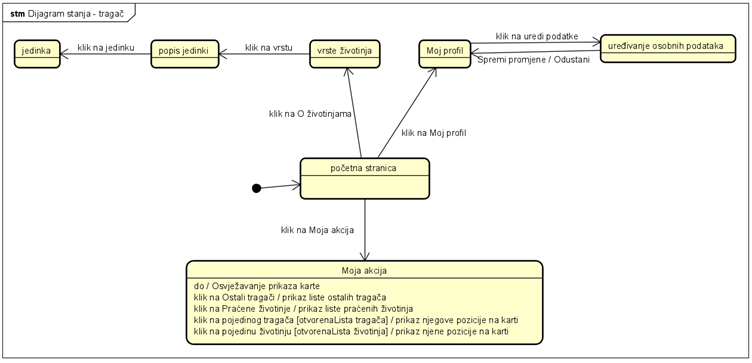
\includegraphics[scale=1]{slike/dijagram stanja - tragač.png}
			\centering
			\caption{Dijagram stanja - tragač}
			\label{fig:dijagram stanja - tragač}
		\end{figure}
			
			\eject 
		
		\section{Dijagram aktivnosti}

		Dijagramom aktivnosti na slici  \ref{fig:dijagram aktivnosti - stvaranje nove akcije} modelirano je stvaranje nove akcije korisnika u ulozi istraživača.
		Do postupka stvaranja nove akcije dolazi se sa stranice prikaza popisa akcija klikom na 
		\textit{Stvori novu akciju}. Na formularu za novu akciju se prilikom klika na \textit{Stvori novu akciju},
		prije spremanja podataka nove akcije u bazu, provjerava jesu li uneseni svi potrebni podatci i jesu li uneseni podatci ispravni.
		Nakon uspješnog stvaranja nove akcije, korisniku se prikazuje osvježen popis akcija, a ukoliko korisnik odustane od stvaranja nove akcije klikom na 
		\textit{Odustani} prikaz se vraća na popis akcija.

		\begin{figure}[H]
			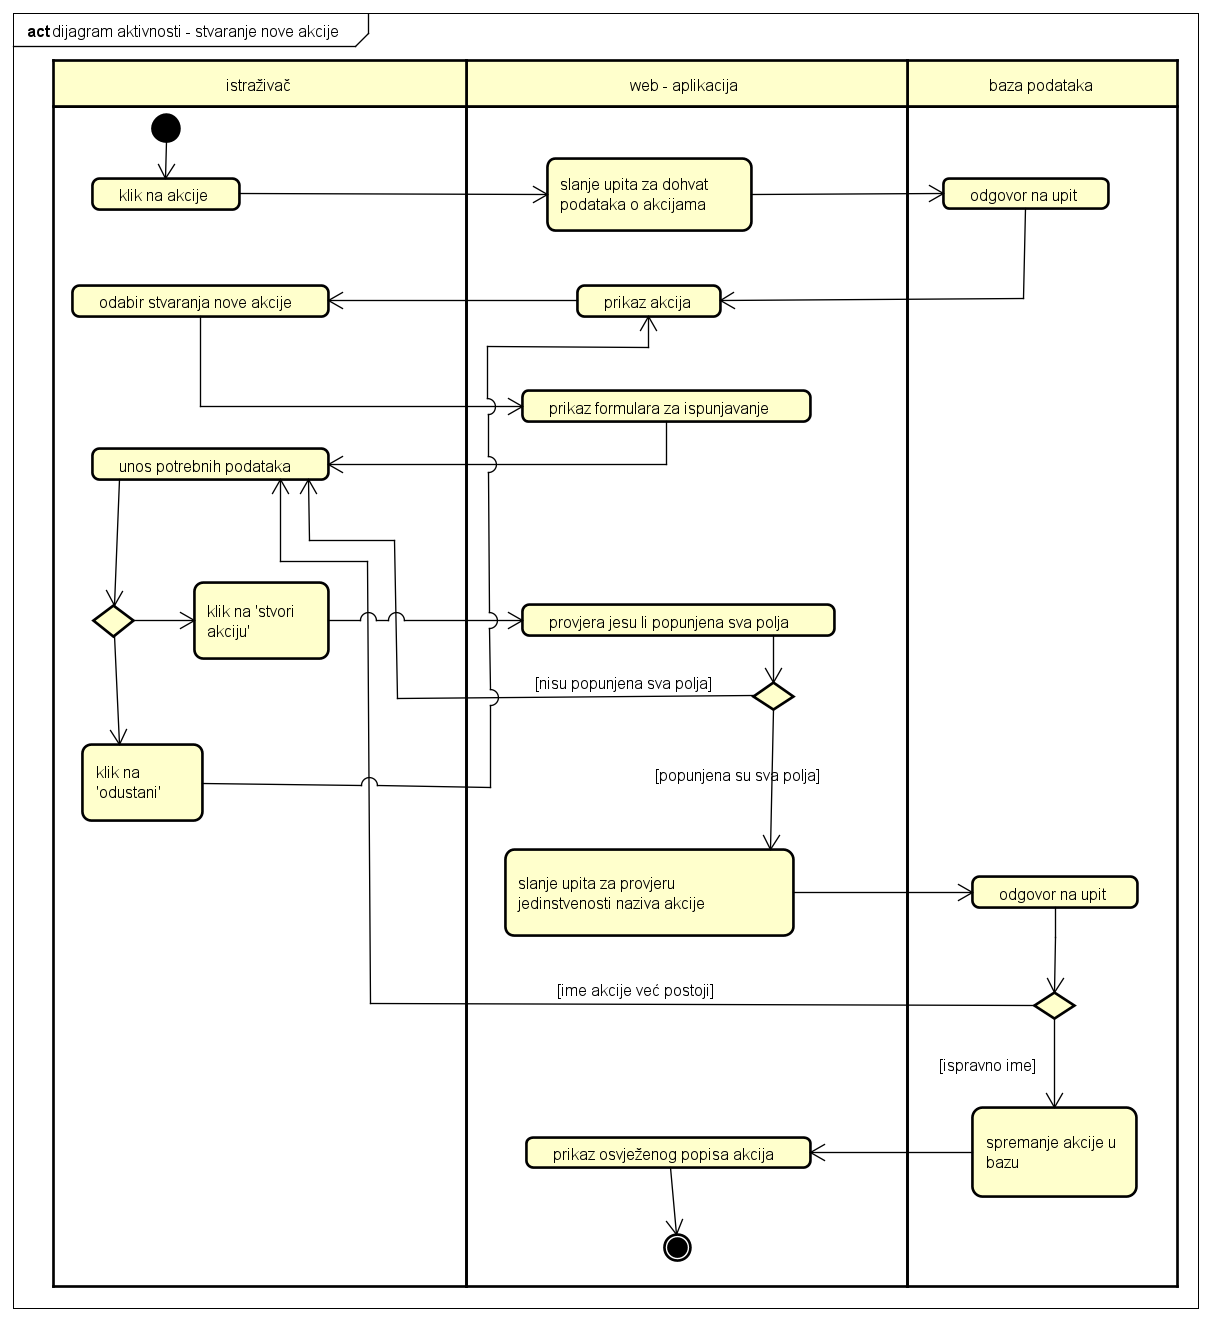
\includegraphics[scale=0.5]{slike/dijagram aktivnosti - stvaranje nove akcije.png}
			\centering
			\caption{Dijagram aktivnosti - stvaranje nove akcije}
			\label{fig:dijagram aktivnosti - stvaranje nove akcije}
		\end{figure}

			\eject


		\section{Dijagram komponenti}

		UML-dijagram komponenti je vrsta strukturnog UML-dijagrama koji
		prikazuje organizaciju i odnose komponenti koje čine programsku potporu. Pruža vizualni prikaz
		arhitekture sustava, naglašavajući modularnu strukturu i interakcije između komponenti, interne strukture i okoline.
		\newline Sustavu se pristupa preko dva razlicita sučelja. Preko sučelja za dohvat HTML, CSS i JS datoteka poslužuju se
datoteke koje pripadaju \textit{frontend} dijelu aplikacije. Router je komponenta koja na
upit s url određuje koja datoteka će se poslužiti na sučelje. Frontend dio se sastoji
od niza JavaScript datoteka koje su raspoređene u logičke cjeline nazvane po tipovima aktora koji im pristupaju. Sve JavaScript datoteke ovise o React biblioteci iz
koje dohvaćaju gotove komponente kao što su gumbi, forme i slično. Preko sučelja 
za dohvat JSON podataka pristupa se REST API komponenti. REST API poslužuje
podatke koji pripadaju \textit{backend} dijelu aplikacije. JpaRepository je sučelje Spring Data JPA projekta korišteno
za jednostavan dohvat i manipulaciju s podacima u bazi podataka, pružajući apstrakciju nad JPA 
(Java Persistence API) omogućavajući  izvođenje operacija nad entitetima bez potrebe za izravnim pisanjem SQL upita. Podaci koji su pristigli 
iz baze se šalju dalje MVC arhitekturi u obliku DTO  (Data transfer object). 
React-view komponenta preko dostupnih sučelja komunicira sa \textit{WildTrack} aplikacijom
te ovisno o korisnikovim akcijama osvježava prikaz i dohvaća nove podatke ili datoteke.
		
		\begin{figure}[H]
			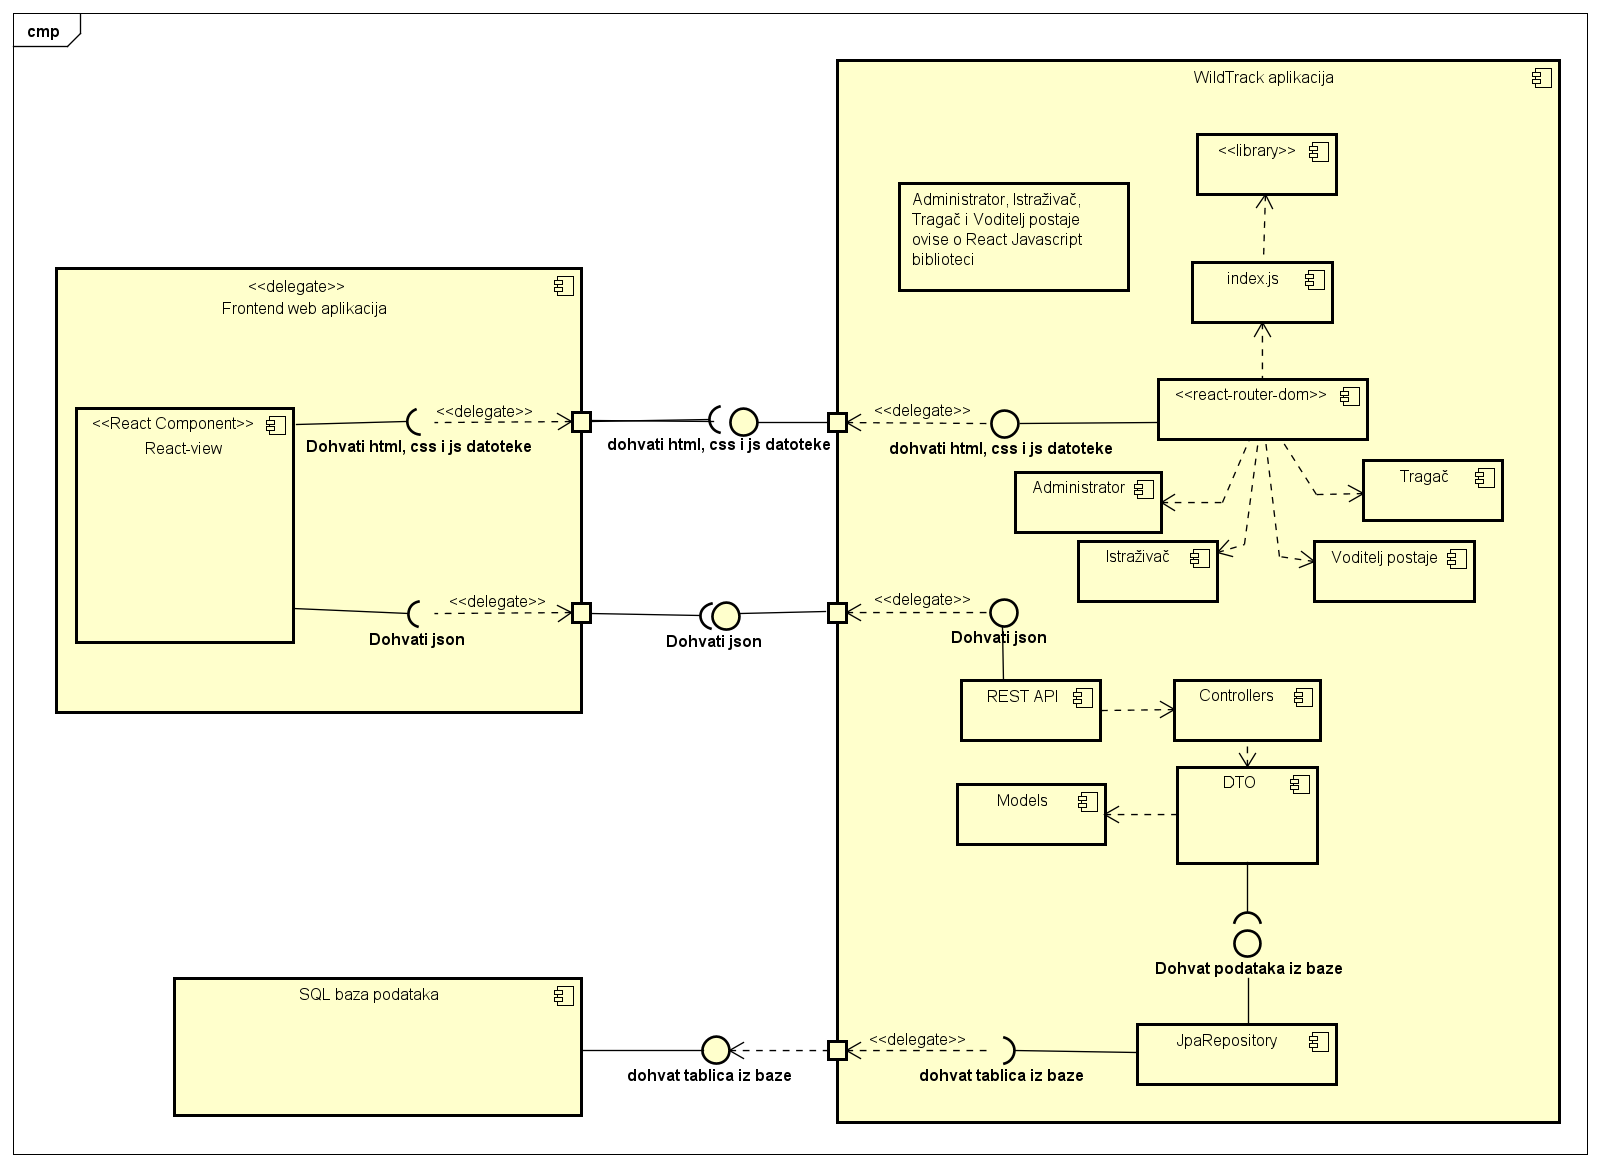
\includegraphics[scale=0.4]{slike/dijagram komponenti.png}
			\centering
			\caption{Dijagram komponenti}
			\label{fig:dijagram komponenti}
		\end{figure}